\section{Datenbankmodelle}
\label{datenmodelle}
In diesem Abschnitt werden die Grundlagen des Graph-basierten Datenbankmodells skizziert. Dieses Graphmodell ist im Rahmen dieser Arbeit von wesentlicher Bedeutung. Schließlich vereint die in \autoref{chap:db2graph} beschriebene Graph-Erweiterung, Elemente des relationalen und Graph-basierten Datenbankmodells. Grundkenntnisse über das relationalen Modell werden dabei hingegen im Rahmen dieser Arbeit vorausgesetzt. Sollten keine Grundkenntnisse über relationale Datenbanksysteme vorhanden sein, empfehlen sich \cite{rdbms_book} und \cite{codd_relational_model} als Einstieg.

Um die Grundlagen des Graphmodells in diesem Abschnitt zu vermittelten, werden die folgenden Aspekte des Modells angesprochen:
\begin{itemize}
    \item Herkunft und Verbreitung,
    \item Struktur und Schema.
\end{itemize}
Die Beschränkung auf diese Aspekte wurde dabei vorgenommen, da die Erläuterung weiterer Aspekt über den Rahmen dieser Arbeit hinausgehen würde. 

Anschließend findet eine kurze Gegenüberstellung des Graphmodells mit dem relationalen Modell statt. Im nächsten Unterabschnitt wird auf die Abfragesprachen von relationalen und Graphdatenbanksystemen eingegangen.

Zum Schluss werden die Informationen nochmals kurz zusammengefasst. 

\subsection{Herkunft und Verbreitung}
Das Graphmodell als Datenbankmodell hat seinen Ursprung in der heutigen Form im Jahr 1999 \cite{gdbms}. Laut 

Dabei wurde das Graphmodell mit der Motivation entwickelt, vermeintliche Nachteile oder Probleme des relational Modells auszuräumen \cite{gdbms}.

Graphdatenbanksysteme und das Graphmodell sind heute als vergleichbar junge Technologien noch nicht so weit verbreitet wie beispielsweise, dass relationale Modell. Mit 1,7 \% der Ranking-Punkte in \cite{db_engines_ranking_july} ordnen sich Graphdatenbanksysteme dabei noch weit hinter anderen Technologien ein, wie \textit{Document Stores}, \textit{Key-Values Stores} oder \textit{Wide column stores} \cite{db_engines_ranking_july} (\autoref{fig:dbms_marketshare}). Jedoch haben Graphdatenbanksysteme seit 2013 laut \cite{db_engines_ranking_july} erheblichen Aufschwung in ihrer Popularität erfahren. So weist diese Datenbanksystemkategorien dort für den Zeitraum 01.2013 bis 07.2021 eine Verhundertfachung des Popularitäts-Score auf \cite{db_engines_ranking_july}. 

\begin{figure}[ht]
    \centering
    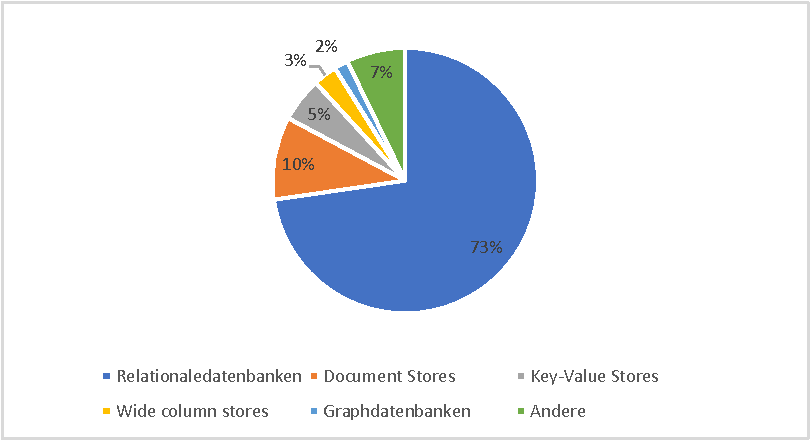
\includegraphics[width=\textwidth]{images/marketshare_dbms.pdf}
    \caption[Anteil Ranking-Punkte nach Datenbankkategorie]{Anteil an Ranking-Punkten nach Datenbankkategorie}
    \label{fig:dbms_marketshare}
    \vspace{1em}
    \textit{Bei den hier abgebildeten Werten handelt es sich um die aufgerundeten Werte aus} \cite{db_engines_ranking_july}\textit{.}
\end{figure}

\subsection{Struktur und Schema}
\label{datenmodelle:structure}
Die Grundlage des Graphmodells stellen sogenannte Knoten und Kanten dar (\textit{engl. Vertexes oder Vertices}) und Kanten (\textit{engl. Edges}) dar. Bei einem Graph handelt es sich hierbei um eine Menge an Knoten und Kanten \cite{gdbms}. In einem solchen Graphen werden dabei Entitäten als Knoten repräsentiert, wie zum Beispiel \textit{Robin} oder \textit{ID3} in \autoref{fig:beispiel_graph}. Die Kanten repräsentieren hingegen, in welcher Beziehung diese Entitäten zueinander stehen. Dies lässt sich gut an den Kanten \textit{besitzt}, \textit{besaß} oder \textit{kennt} in \autoref{fig:beispiel_graph} nachvollziehen. Wie in \autoref{fig:beispiel_graph} auch erkennbar ist, verfügen die Kanten dabei immer über eine Richtung. Also einen Start- und einen Zielknoten den sie verbinden. 

Knoten und Kanten können dabei in diesem Modell anhand von sogenannten Labels organisiert werden. So können Knoten oder Kanten, die eine ähnliche Rolle einnehmen, dieselben Labels zugewiesen werden. Die Verwendung von Labels wird hierbei in \autoref{fig:beispiel_graph} durch die unterschiedlichen Farben gekennzeichnet. So werden darin die als Auto gelabelten Knoten in hellbraun markiert, während die Personen rot eingefärbt werden. 

Das Graphmodell setzt, anders als das relationale Modell, auf ein flexibles Datenbankschema \cite{gdbms}. Durch dieses flexible Schema fällt es leicht heterogene Daten in dem Graphmodell abzubilden. 

\begin{figure}[ht]
    \centering
    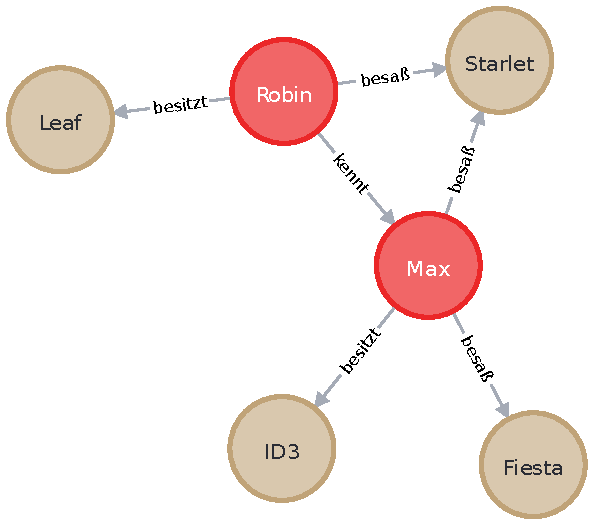
\includegraphics[width=0.75\textwidth]{images/example_graph.pdf}
    \caption{Beispiel Graph}
    \vspace{1em}
    \textit{Hier wird ein Beispiel Graph abgebildet der die Besitzbeziehungen zwischen einer Person (Besitzer) und einem Auto modelliert.}
    \label{fig:beispiel_graph}
\end{figure}

\subsection{Vergleich}
In diesem Unterabschnitt findet ein kleiner Vergleich zwischen dem Graph-basierten und relationalen Datenmodell statt. Dieser kann als kurze Übersicht angesehen werden, der die wichtigsten Unterschiede zwischen den Datenbankmodellen aufführt. 

In der folgenden Aufzählung werden dabei die drei wichtigsten Unterschiede zwischen den Datenmodellen angesprochen:
\begin{itemize}
    \item Das Graphmodell verfügt über ein flexibles Schema, während beim relationalen Modell auf ein striktes Schema gesetzt wird \cite{gdbms,rdbms_book}.
    \item Im relationalen Modell werden alle Informationen in Tabellen abgelegt \cite{rdbms_book}. Im Graphmodell werden die Daten in Knoten und Kanten gehalten \cite{gdbms}. 
    \item Beziehungen werden in einem Graphdatenbanksystem durch Kanten zwischen einem Start- und Zielknoten repräsentiert \cite{gdbms}. Beim relationalen Modell werden Beziehungen durch die Referenzierung eines Primärschlüssels einer anderen Tabelle vorgenommen \cite{rdbms_book}. 
\end{itemize}
Bei der genaueren Betrachtung der Unterschiede aus der vorausgegangenen Aufzählung fällt jedoch auf, dass diese auch als Ähnlichkeiten betrachtet werden können. So verfügen beide Modelle trotz ihrer unterschiedlichen Herangehensweise über ein Schema, besitzen Strukturen in denen Informationen gehalten werden und bieten die Möglichkeit Beziehungen abzubilden. Somit scheinen die beiden Modell zumindest bezüglich dieser Aspekte äquivalent zu sein. Schließlich verfügen beide Datenmodelle über Strukturen und Mechanismen, um Daten zu halten und Beziehung zu modellieren. 

Wenn nun allerdings beide Datenmodelle über die Mittel verfügen, Daten zu halten und Beziehungen abzubilden, stellt sich die Frage: \textit{Wann sollte welches Datenmodell herangezogen werden?}

Die ausführliche Beantwortung dieser Frage würde hierbei einmal mehr den Rahmen der Arbeit sprengen. Allerdings können die beiden folgenden Szenarien kleine Einblicke dazu geben. 

\subsubsection{Szenario 1.}
In diesem Szenario wird auf Queries eingegangen bei denen Beziehungen beziehungsweise der Beziehungsgrad eine wichtige Rolle spielen. 

Hierfür wird eine Angestelltenhierarchie eines Unternehmens herangezogen. Bei den Daten, die die Modelle hierbei repräsentieren sollen, handelt es sich um einen Datensatz an Angestellten. Diese angestellten verfügen hierbei wie in \autoref{fig:angestellten_tabelle} und \autoref{fig:angestellten_graph} erkennbar über einen Namen und einen Vorgesetzten, dem sie unterstellt sind. 

Nun soll in diesem Szenario ermittelt werden, wer \textit{Alice} Vorgesetzter dritten Grades in diesem Unternehmen ist. Also wer der Vorgesetzte des Vorgesetzten des Vorgesetzten von \textit{Alice} ist. Bei dem Graphen in \autoref{fig:angestellten_tabelle} kann dies leicht nachvollzogen werden. Es muss lediglich dreimal den \texttt{hat\_vorgesetzten}-gelabelten Kanten gefolgt werden, bis der Zielknoten \textit{Dave} erreicht wird. 

\begin{figure}[ht]
    \centering
    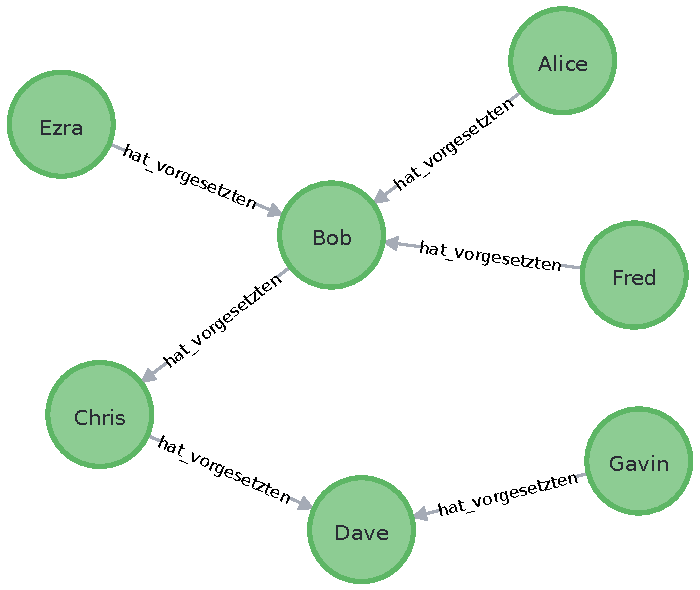
\includegraphics[width=0.8\textwidth]{images/angestellten_graph.pdf}
    \caption{Angestelltenhierarchie Graph}
    \label{fig:angestellten_graph}
\end{figure}

Bei \autoref{fig:angestellten_tabelle} ist der Aufwand jedoch etwas höher. Hier müssen für die Ermittlung des Namen des Vorgesetzten dritten Grades mindestens zwei Joins der Tabelle mit sich selbst durchgeführt werden. Dies stellt bei den kleinen Tabellen und dem niedrigen Grad im Anwendungsfall noch kein Problem dar. Bei einem größeren Datensatz oder einem höheren Grad würden beide Faktoren die Last und Performance des Datenbanksystems stark beeinträchtigen. Schließlich sind solche rekursiven Joins Ressourcen-intensiv, besonders wenn zwei große Tabellen gejoined werden \cite{gdbms}. 

\begin{figure}[ht]
    \centering
    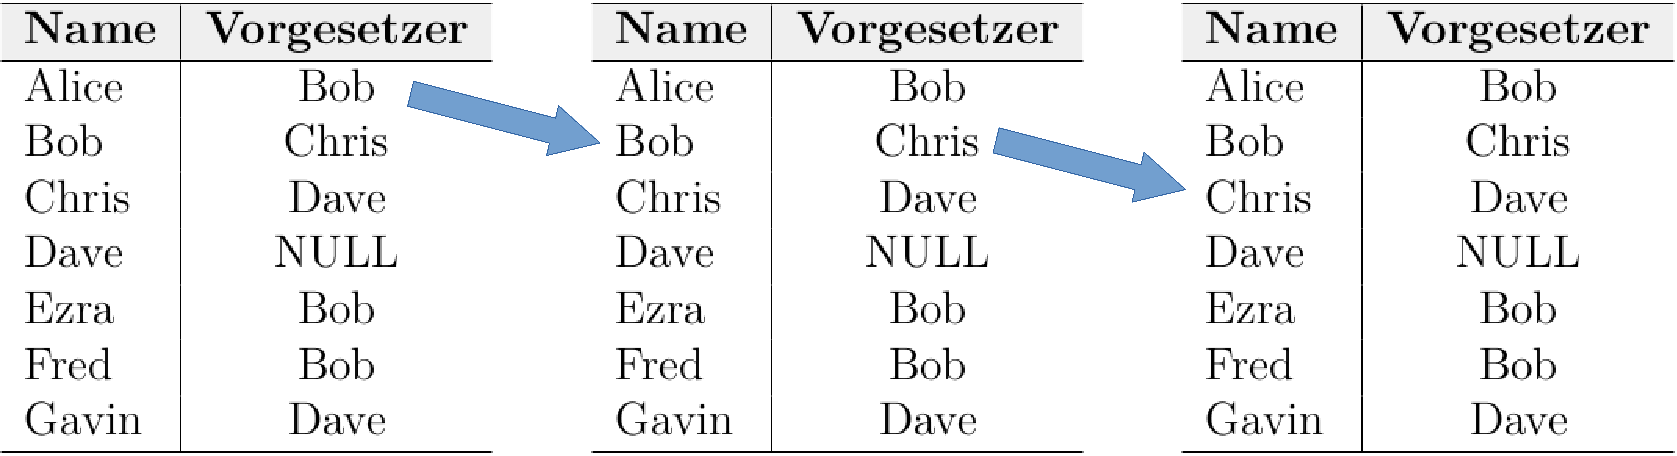
\includegraphics[width=\textwidth]{images/angestellte_tabellen.pdf}
    \caption{Angestelltenhierarchie Tabelle}
    \label{fig:angestellten_tabelle}
\end{figure}

\subsubsection{Szenario 2.}


\section{Abfragesprachen}
In diesem Abschnitt wird auf die für die Arbeit relevanten Abfragesprachen:
\begin{itemize}
    \item SQL,
    \item Gremlin und
    \item Cypher eingegangen.
\end{itemize}
Ziel dieses Abschnittes ist es dabei eine kleine Übersicht über die Abfragesprachen zu geben, die im Kontext dieser Arbeit eine besondere Rolle spielen. Abschließend werden die wichtigsten Punkte des Abschnitts nochmal kurz zusammengefasst.

\subsection{SQL}
Bei SQL handelt es sich um eine Abfragesprache, die im Feld der relationalen Datenbanksysteme weit verbreitet ist \cite{sql_history}. Sie wurde von Donald D. Chamberlin und Raymond F. Boyce im Rahmen des \textit{System R} Projekts entwickelt \cite{sql_history}. SQL wurde dabei mit der Motivation entworfen eine einfache Abfragesprache für relationale Daten zu entwickeln \cite{sql_history}. 

SQL selbst stellt hierbei eine deklarative Abfragesprache dar \cite{sql_history}. Der grundlegende Aufbau der Sprache und die Syntax können dabei \autoref{src:sql_example} entnommen werden. So ist in \autoref{src:sql_example} klar erkennbar, dass sich alle Operationen auf Tabellen und Spalten beziehen. Die Sprache arbeitet also -- wie erwartet -- in den Strukturen des relationalen Modells.

\begin{lstlisting}[caption={Beispiel SQL-Queries},language=SQL,label=src:sql_example]
/* Tabelle erstellen */
CREATE TABLE Autos (
    Fahrzeugnummer VARCHAR(50), 
    Marke VARCHAR(10), 
    Modell VARCHAR(10), 
    Baujahr INT,
    PRIMARY KEY(Fahrzeugnummer)
);

/* Daten in Tabelle schreiben */
INSERT INTO Autos 
(Fahrzeugnummer, Marke, Modell, Baujahr) 
("FZ-123456789", "Toyota", "Starlet", 1997);

/* Daten Abfragen */
SELECT Marke, Model, Baujahr FROM Autos 
WHERE Fahrzeugnummer = "FZ-123456789";

/* Daten Loeschen */
DELETE FROM Autos WHERE Fahrzeugnummer = "FZ-123456789";
\end{lstlisting}

Des Weiteren muss darauf hingewiesen werden, dass SQL als Sprache standardisiert wurde \cite{sql_history}. Allerdings gibt es heute trotz des Standards weiterhin sogenannte SQL-Dialekte \cite{sql_2017}. So können sich einige SQL Sprachelemente je nach Datenbanksystem oder Hersteller weiterhin unterscheiden \cite{sql_2017}. 

\subsection{Gremlin}

Bei Gremlin handelt es sich um eine Abfragesprache die für  Graphdatenbanksystemen \cite{tinkerpop_2020}. Die Sprache steht dabei in direkter Verbindung mit dem TinkerPop Projekt  \cite{tinkerpop_2020}. Zu den Datenbanksystemen, die die Abfragesprache nutzen, gehört neben Db2 Graph, das im Rahmen der Arbeit eine wichtige Rolle spielt, gehören auch:
\begin{itemize}
    \item JanusGraph \cite{janusgraph_2020},
    \item Amazon Neptune \cite{neptune_2021} und 
    \item CosmosDB von Microsoft \cite{cosmosdb_2021}.
\end{itemize}

Für die Interaktion mit den Graphen bietet Gremlin dabei zwei verschiedene Abfragestile \cite{gremlin_paper}. So ist es einerseits möglich imperativ einen sogenannten Graph-Traversal durchzuführen, um mit dem Graph zu interagieren \cite{gremlin_paper}. Anderseits ist es allerdings auch möglich einen deklarativen Pattern-Matching-Stil zu wählen \cite{gremlin_paper}. Im Rahmen dieser Arbeit wurde bei Gremlin-Queries immer der imperative Graph-Traversal basierte Ansatz gewählt \cite{gremlin_paper}. Daher werden als Beispiel in \autoref{src:gremlin_example} lediglich imperative Queries aufgeführt. 

\begin{lstlisting}[caption={Beispiel Gremlin-Queries},language=JAVA,label=src:gremlin_example]
/* Daten in den Graph einfuegen */
v1 = g.addV('Auto').property('Modell','Leaf');
v2 = g.addV('Person').property('Name','Robin');
g.V(v1).addE('besitzt').to(v2).property('seit', '2019.08.08');

/* Daten abfragen */
g.V().hasLabel('Person').has('Name','Robin').outE('besitzt').outV().values('Modell')

/* Daten loeschen */
g.V().hasLabel("Person").has('Name', 'Max').drop();
\end{lstlisting}

\subsection{Cypher}
Die Abfragesprache Cypher, wurde mit dem Ziel entworfen eine einfache, deklarative Art der Interaktion mit Graph-Daten zu ermöglichen \cite{gdbms}. Eine wichtige Sprachkomponente stellt dabei der Pattern-Matching-Stiel dar \cite{gdbms}. Von den beiden für die Arbeit relevanten Datenbanksystemen Neo4j und Db2 Graph unterstützt allerdings nur Neo4j die Sprache -- zumindest direkt. 

In \autoref{src:cypher_example} werden hierbei einige Beispiel-Cypher-Queries aufgeführt. Diese sind mit den Gremlin-Queries in \autoref{src:gremlin_example} bezüglich ihrer Funktion vergleichbar. 

\begin{lstlisting}[caption={Beispiel Cypher-Queries},language=SQL,label=src:cypher_example]
/* Daten in den Graph einfuegen */
CREATE (:Person{name: "Robin"})-[:besitzt{seit: "2019.08.08"}]->(:Auto{modell: "Leaf"});

/* Daten abfragen */
MATCH (:Person{name: "Robin"})-[:besitzt]->(n2) RETURN n2.modell;

/* Daten loeschen */
MATCH (n:Person{name: "Robin"}) DETACH DELETE n;
\end{lstlisting}

Neben Neo4j das im Kontext der Arbeit eine wichtige Rolle spielt unterstützen auch die Datenbanksysteme:
\begin{itemize}
    \item RedisGraph \cite{redisgraph_2021},
    \item SAP HANA Graph \cite{opencypher_2021} und
    \item Agens Graph \cite{opencypher_2021}.
\end{itemize}

\subsection{Zusammenfassung}
Bei den im Rahmen der Arbeit relevanten Abfragesprachen handelt es sich um SQL, Gremlin und Cypher. 

SQL stellt dabei eine Abfragesprache für relationale Datenbanksysteme dar, während Gremlin und Cypher für den Einsatz bei Graphdatenbanksystemen konzipiert wurden. 

Bei SQL und Cypher handelt es sich um deklarative Abfragesprachen. Gremlin hingegen neben einem imperativen Abfragestil auch eine deklarative Art Queries zu formulieren. 